% this file is called up by thesis.tex
% content in this file will be fed into the main document

\chapter{A review in Social Media Authentication} % top level followed by section, subsection

% change according to folder and file names
\ifpdf
    \graphicspath{{X/figures/PNG/}{X/figures/PDF/}{X/figures/}}
\else
    \graphicspath{{X/figures/EPS/}{X/figures/}}
\fi

% ----------------------- State of the art ------------------------


\section{Authentication Process Usability}
Authentication process usability in this context refers to automating or simplifying the process of authenticating the user accessing the phone or features on the phone. This section discusses some of the tools used on mobile phones or tablets to simplify authentication.

\subsection{Android AccountManager}
Most of the applications are using Android AccountManager \footnote[4]{http://developer.android.com/intl/zh-CN/reference/android/accounts/AccountManager.html}, see Figure 2.1, as a tool to automate authentication. It is a built in centralized registry that can hold user credentials or even authentication tokens which are generated via application server. Though it requires implementing various components, increasing the complexity, it is still a good method for single user device. For example Google \footnote[5]{https://play.google.com/store/apps/ - Google}, Facebook \footnote[6]{https://play.google.com/store/apps/ - Facebook}, and Microsoft Outlook \footnote[7]{https://play.google.com/store/apps/ - Microsoft Office Outlook} each use this method. 

\begin{figure}
\centering
\begin{minipage}{.5\textwidth}
  \centering
  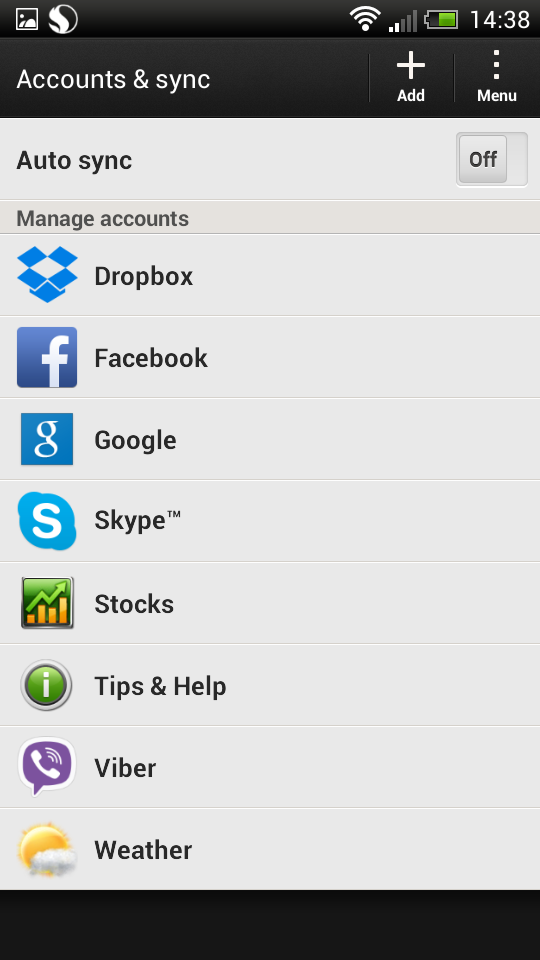
\includegraphics[width=.6\linewidth]{images/accountmanager.png}
  \captionof{figure}{Android AccountManager}
  \label{fig:android accountmanager}
\end{minipage}%
\begin{minipage}{.5\textwidth}
  \centering
  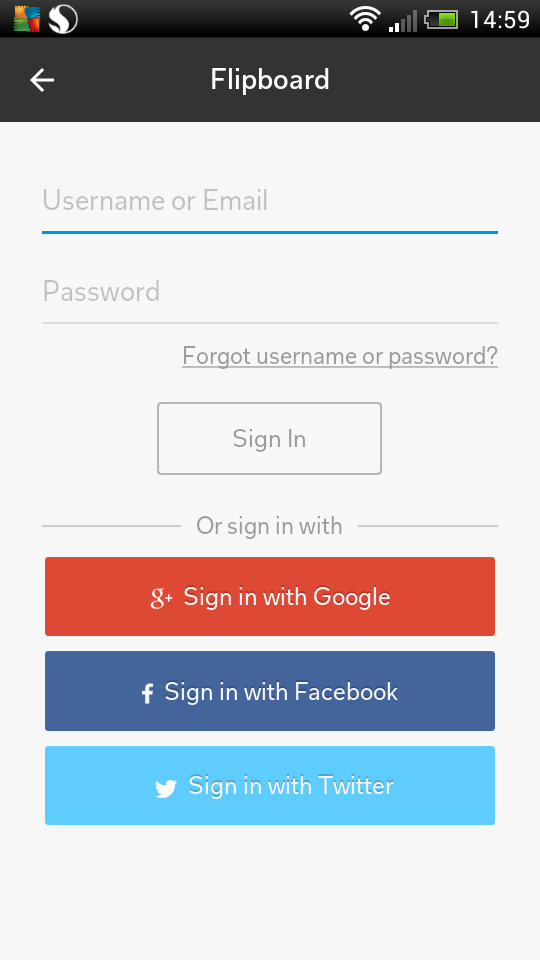
\includegraphics[width=.6\linewidth]{images/facebookgoogletwitter.png}
  \captionof{figure}{Service providers}
  \label{fig:google identity platform, facebook sdk}
\end{minipage}
\end{figure}

\subsection{Service providers}
The next most used method of authentication is provided by social media websites. These providers are giving developers the option to let users authenticate by using accounts on the social media websites. Users do not have to create new accounts to these sites, but will refer to their already existing accounts on social media as a way of registration. On android the user needs to have that social media application installed and logged in to use this method. The most known two providers are Google and Facebook. As an example of how service provider tools appear on an application, ''Flipboard: Your New Magazine'' \footnote[8]{https://play.google.com/store/apps/ - Flipboard: Your News Magazine} app is used, seen on Figure 2.2.

\subsubsection{Google Identity Platform}
Google is providing android developers with an application programming interface (API) which allows users to register and authenticate using Google account, but also allows developers to integrate other Google services into their applications: payments via Google Wallet, sharing with Google+, saving files to Drive, etc. \footnote[9]{https://developers.google.com/identity/}

\subsubsection{Facebook SDK}
Facebook has a software development kit (SDK) for android developers. Just as with Google API, the SDK allows authentication via Facebook account and also provides more services - sharing on Facebook, sending application invites via Facebook, etc. \footnote[10]{https://developers.facebook.com/docs/android}

\section{Previous research}

\subsection{Visual login}
Visual login refers to a class of mechanisms that rely on the selection of icons or photo images to produce a
password value. Visual login is a knowledge-based approach like passwords. Instead of alphanumeric characters, users must remember image sequences. Visual images are presented to the user for selection by tiling a portion of the user's graphical interface window with identically sized squares, grouped into a 5 x 6 matrix. The surface of each square displays a bit-mapped image or thumbnail of some picture supplied in a predefined digital format. Selecting the correct sequence of thumbnail images authenticates the user to the device. \cite{jansen2003authenticating}

\subsection{Tap pattern}
Gesture interaction with mobile devices has become common-place. One class of gestures that is widely used is tapping. While key strokes are usually perceived as single events, taps have an implied duration in time. Single taps, long presses and double taps are common examples. These simple patterns can be detected efficiently with very crude algorithms, relying solely on timers. Tap patterns, however, can be more generally defined as a sequence of intervals of ''on'' and ''off'' times that is, the ordered time distances between and within taps. \cite{marques2013under}

\subsection{Fingerphoto recognition}
The intention of the fingerphoto recognition is that for authentication the user simply positions his finger close in front of the camera in order to capture a biometric sample. The algorithms for finger detection and quality assurance check continuously the preview images of the camera after the capture process has been initiated by the user. The results of the algorithms are calculated in real-time and are displayed on the graphical user interface. A photo is automatically taken when all criteria for the fingerphoto recognition are fulfilled. \cite{stein2012fingerphoto}

\subsection{Token-based authentication}
Authentication on smartphones does not have to include doing something to or with the device, instead it can involve a physical token. The token can be so small it could be carried on a key chain and it automatically unlocks the smartphone whenever its owner wants to use it. The token is based on magnetic fields detected by the smartphone's compass or on an acoustic transmitter that generates a signal picked up by the handset's microphone. All the user has to do is carry the token with him. \cite{bojinov2011mobile}

\subsection{Arm's flex}
One of the human behaviors considered being unique is arm's flex. It is a gestural pattern i.e. the way people bend their arm for picking a phone when responding to incoming calls. That arm's flexing is considered as a subset of gesture pattern in lower limb gesture. Every person who bends their arm will have different strength measured by accelerometer using smartphone even if they own same arm's flex pattern visually.\cite{negara2012arm, srirama2011zompopo}

\subsection{Multitouch image-based authentication}
Multitouch image-based authentication password can consist of multiple rounds, where in each round the user can mark multiple points on an image. Click points have the advantage that they can be entered quickly,  even with multiple fingers simultaneously, while drawing complex patterns requires more time. Multitouch authentication uses background images as cues and determines the image for the next round based on the user's input in the current round. Thus, the user can instantly recognize if the points selected in the previous round were correct or wrong (expected vs. unexpected image in next round). A back button allows for correction of errors. Each image should also only appear once in a password sequence to prevent memory interference between two instances of the same image. \cite{ritter2013miba}

\section{Continous authentication}
It is not always good to have a phone authenticate the user once and let him keep using the phone till it gets locked automatically by a timer or physically by the user. Hence there are methods that monitor the phone even when the phone is unlocked and only when there is sufficient evidence that the current user is not the smartphone owner, traditional user authentication is activated. The next sections describe continous authentication methods.

\subsection{Gait recognition}
The term gait recognition describes a biometric method
which allows an automatic verification of the identity of a person by the way he walks. Gait recognition is based on wearing motion recording sensors on the body in different places: on the waist, in pockets. The wearable sensors can be accelerometers (measuring acceleration), gyro sensors (measuring rotation and number of degrees per second of rotation), force sensors (measuring the force when walking) etc. \cite{derawi2010unobtrusive, srirama2012social}

\subsection{Keystroke analysis}
This method of authentication analysis the detailed timing information that describes exactly when each key was pressed and when it was released by the person typing. \cite{buchoux2008deployment}

\subsection{Location information}
Phones and tablets nowadays come with built-in GPS systems. GPS individually or in cooperation with cell towers allows a phone to acquire its current location which is analysed against previous data.  \cite{takamizawa2012authentication}

\subsection{Orientation sensor}
A user has a unique way to hold and operate his/her smartphone while working on some applications and such behavioral biometrics can be captured from the readings of the orientation sensor. User's behavioral biometrics of up-down flicks and left-right flicks from the orientation sensor are monitored to authenticate. \citep{lin2012new}

\subsection{TouchScreen gestures}
As long as the smartphone is used, gestures are monitored to authenticate the user continuously.
Continuous authentication in done on the background using intercepted touch data from
normal user-smartphone interactions. The detection approach is invoked on-demand whenever touch inputs are received and is transparent to the smartphone user. Selected touch gesture information are collected including gesture type, X and Y coordinates, directions of the finger motion, finger motion speed, pressure at each sampled touch point and the distance between multi-touch points. In total, there are 53 features for each touch gesture. The six most frequent and useful gestures: down to up swipe, up to down swipe, left to right swipe, right to left swipe, zoom-in, and zoom-out. Since a smartphone user may apply different levels of touch pressure at different stages of a touch gesture, they are divided into three segments, (i) the
beginning of a touch motion, (ii) the main touch motion, which
is the longest segment and (iii) the end of a touch motion. \cite{feng2012continuous, li2013unobservable}

\section{Summary}
The world of android and mobile in general is filled with means to authenticate the user. All of the methods discussed have their advantages and disadvantages, but they all serve the same purpose of keeping our device and data secure. The most commonly used methods, Android AccountManager and service providers, accomplish the task of automating authentication well, but either have the user tie their account to some other social media or do not have the support for multiple users. There has been a lot research done on the authentication for mobile, with interesting methods being developed, but so far none of them is considering support for multiple users. The next chapter describes the problem in more detail.



